
%% bare_conf.tex
%% V1.3
%% 2007/01/11
%% by Michael Shell
%% See:
%% http://www.michaelshell.org/
%% for current contact information.
%%
%% This is a skeleton file demonstrating the use of IEEEtran.cls
%% (requires IEEEtran.cls version 1.7 or later) with an IEEE conference paper.
%%
%% Support sites:
%% http://www.michaelshell.org/tex/ieeetran/
%% http://www.ctan.org/tex-archive/macros/latex/contrib/IEEEtran/
%% and
%% http://www.ieee.org/

%%*************************************************************************
%% Legal Notice:
%% This code is offered as-is without any warranty either expressed or
%% implied; without even the implied warranty of MERCHANTABILITY or
%% FITNESS FOR A PARTICULAR PURPOSE! 
%% User assumes all risk.
%% In no event shall IEEE or any contributor to this code be liable for
%% any damages or losses, including, but not limited to, incidental,
%% consequential, or any other damages, resulting from the use or misuse
%% of any information contained here.
%%
%% All comments are the opinions of their respective authors and are not
%% necessarily endorsed by the IEEE.
%%
%% This work is distributed under the LaTeX Project Public License (LPPL)
%% ( http://www.latex-project.org/ ) version 1.3, and may be freely used,
%% distributed and modified. A copy of the LPPL, version 1.3, is included
%% in the base LaTeX documentation of all distributions of LaTeX released
%% 2003/12/01 or later.
%% Retain all contribution notices and credits.
%% ** Modified files should be clearly indicated as such, including  **
%% ** renaming them and changing author support contact information. **
%%
%% File list of work: IEEEtran.cls, IEEEtran_HOWTO.pdf, bare_adv.tex,
%%                    bare_conf.tex, bare_jrnl.tex, bare_jrnl_compsoc.tex
%%*************************************************************************

% *** Authors should verify (and, if needed, correct) their LaTeX system  ***
% *** with the testflow diagnostic prior to trusting their LaTeX platform ***
% *** with production work. IEEE's font choices can trigger bugs that do  ***
% *** not appear when using other class files.                            ***
% The testflow support page is at:
% http://www.michaelshell.org/tex/testflow/



% Note that the a4paper option is mainly intended so that authors in
% countries using A4 can easily print to A4 and see how their papers will
% look in print - the typesetting of the document will not typically be
% affected with changes in paper size (but the bottom and side margins will).
% Use the testflow package mentioned above to verify correct handling of
% both paper sizes by the user's LaTeX system.
%
% Also note that the "draftcls" or "draftclsnofoot", not "draft", option
% should be used if it is desired that the figures are to be displayed in
% draft mode.
%
\documentclass[10pt, conference, compsocconf]{IEEEtran}
\IEEEoverridecommandlockouts
% Add the compsocconf option for Computer Society conferences.
%
% If IEEEtran.cls has not been installed into the LaTeX system files,
% manually specify the path to it like:
% \documentclass[conference]{../sty/IEEEtran}



% Some very useful LaTeX packages include:
% (uncomment the ones you want to load)


% *** MISC UTILITY PACKAGES ***
%
%\usepackage{ifpdf}
% Heiko Oberdiek's ifpdf.sty is very useful if you need conditional
% compilation based on whether the output is pdf or dvi.
% usage:
% \ifpdf
%   % pdf code
% \else
%   % dvi code
% \fi
% The latest version of ifpdf.sty can be obtained from:
% http://www.ctan.org/tex-archive/macros/latex/contrib/oberdiek/
% Also, note that IEEEtran.cls V1.7 and later provides a builtin
% \ifCLASSINFOpdf conditional that works the same way.
% When switching from latex to pdflatex and vice-versa, the compiler may
% have to be run twice to clear warning/error messages.






% *** CITATION PACKAGES ***
%
%\usepackage{cite}
% cite.sty was written by Donald Arseneau
% V1.6 and later of IEEEtran pre-defines the format of the cite.sty package
% \cite{} output to follow that of IEEE. Loading the cite package will
% result in citation numbers being automatically sorted and properly
% "compressed/ranged". e.g., [1], [9], [2], [7], [5], [6] without using
% cite.sty will become [1], [2], [5]--[7], [9] using cite.sty. cite.sty's
% \cite will automatically add leading space, if needed. Use cite.sty's
% noadjust option (cite.sty V3.8 and later) if you want to turn this off.
% cite.sty is already installed on most LaTeX systems. Be sure and use
% version 4.0 (2003-05-27) and later if using hyperref.sty. cite.sty does
% not currently provide for hyperlinked citations.
% The latest version can be obtained at:
% http://www.ctan.org/tex-archive/macros/latex/contrib/cite/
% The documentation is contained in the cite.sty file itself.






% *** GRAPHICS RELATED PACKAGES ***
%
\ifCLASSINFOpdf
  \usepackage[pdftex]{graphicx}
  % declare the path(s) where your graphic files are
  % \graphicspath{{../pdf/}{../jpeg/}}
  % and their extensions so you won't have to specify these with
  % every instance of \includegraphics
  % \DeclareGraphicsExtensions{.pdf,.jpeg,.png}
\else
  % or other class option (dvipsone, dvipdf, if not using dvips). graphicx
  % will default to the driver specified in the system graphics.cfg if no
  % driver is specified.
  % \usepackage[dvips]{graphicx}
  % declare the path(s) where your graphic files are
  % \graphicspath{{../eps/}}
  % and their extensions so you won't have to specify these with
  % every instance of \includegraphics
  % \DeclareGraphicsExtensions{.eps}
\fi
% graphicx was written by David Carlisle and Sebastian Rahtz. It is
% required if you want graphics, photos, etc. graphicx.sty is already
% installed on most LaTeX systems. The latest version and documentation can
% be obtained at: 
% http://www.ctan.org/tex-archive/macros/latex/required/graphics/
% Another good source of documentation is "Using Imported Graphics in
% LaTeX2e" by Keith Reckdahl which can be found as epslatex.ps or
% epslatex.pdf at: http://www.ctan.org/tex-archive/info/
%
% latex, and pdflatex in dvi mode, support graphics in encapsulated
% postscript (.eps) format. pdflatex in pdf mode supports graphics
% in .pdf, .jpeg, .png and .mps (metapost) formats. Users should ensure
% that all non-photo figures use a vector format (.eps, .pdf, .mps) and
% not a bitmapped formats (.jpeg, .png). IEEE frowns on bitmapped formats
% which can result in "jaggedy"/blurry rendering of lines and letters as
% well as large increases in file sizes.
%
% You can find documentation about the pdfTeX application at:
% http://www.tug.org/applications/pdftex





% *** MATH PACKAGES ***
%
\usepackage[cmex10]{amsmath}
% A popular package from the American Mathematical Society that provides
% many useful and powerful commands for dealing with mathematics. If using
% it, be sure to load this package with the cmex10 option to ensure that
% only type 1 fonts will utilized at all point sizes. Without this option,
% it is possible that some math symbols, particularly those within
% footnotes, will be rendered in bitmap form which will result in a
% document that can not be IEEE Xplore compliant!
%
% Also, note that the amsmath package sets \interdisplaylinepenalty to 10000
% thus preventing page breaks from occurring within multiline equations. Use:
\interdisplaylinepenalty=2500
% after loading amsmath to restore such page breaks as IEEEtran.cls normally
% does. amsmath.sty is already installed on most LaTeX systems. The latest
% version and documentation can be obtained at:
% http://www.ctan.org/tex-archive/macros/latex/required/amslatex/math/





% *** SPECIALIZED LIST PACKAGES ***
%
%\usepackage{algorithmic}
% algorithmic.sty was written by Peter Williams and Rogerio Brito.
% This package provides an algorithmic environment fo describing algorithms.
% You can use the algorithmic environment in-text or within a figure
% environment to provide for a floating algorithm. Do NOT use the algorithm
% floating environment provided by algorithm.sty (by the same authors) or
% algorithm2e.sty (by Christophe Fiorio) as IEEE does not use dedicated
% algorithm float types and packages that provide these will not provide
% correct IEEE style captions. The latest version and documentation of
% algorithmic.sty can be obtained at:
% http://www.ctan.org/tex-archive/macros/latex/contrib/algorithms/
% There is also a support site at:
% http://algorithms.berlios.de/index.html
% Also of interest may be the (relatively newer and more customizable)
% algorithmicx.sty package by Szasz Janos:
% http://www.ctan.org/tex-archive/macros/latex/contrib/algorithmicx/




% *** ALIGNMENT PACKAGES ***
%
\usepackage{array}
% Frank Mittelbach's and David Carlisle's array.sty patches and improves
% the standard LaTeX2e array and tabular environments to provide better
% appearance and additional user controls. As the default LaTeX2e table
% generation code is lacking to the point of almost being broken with
% respect to the quality of the end results, all users are strongly
% advised to use an enhanced (at the very least that provided by array.sty)
% set of table tools. array.sty is already installed on most systems. The
% latest version and documentation can be obtained at:
% http://www.ctan.org/tex-archive/macros/latex/required/tools/


%\usepackage{mdwmath}
%\usepackage{mdwtab}
% Also highly recommended is Mark Wooding's extremely powerful MDW tools,
% especially mdwmath.sty and mdwtab.sty which are used to format equations
% and tables, respectively. The MDWtools set is already installed on most
% LaTeX systems. The lastest version and documentation is available at:
% http://www.ctan.org/tex-archive/macros/latex/contrib/mdwtools/


% IEEEtran contains the IEEEeqnarray family of commands that can be used to
% generate multiline equations as well as matrices, tables, etc., of high
% quality.


%\usepackage{eqparbox}
% Also of notable interest is Scott Pakin's eqparbox package for creating
% (automatically sized) equal width boxes - aka "natural width parboxes".
% Available at:
% http://www.ctan.org/tex-archive/macros/latex/contrib/eqparbox/





% *** SUBFIGURE PACKAGES ***
%\usepackage[tight,footnotesize]{subfigure}
% subfigure.sty was written by Steven Douglas Cochran. This package makes it
% easy to put subfigures in your figures. e.g., "Figure 1a and 1b". For IEEE
% work, it is a good idea to load it with the tight package option to reduce
% the amount of white space around the subfigures. subfigure.sty is already
% installed on most LaTeX systems. The latest version and documentation can
% be obtained at:
% http://www.ctan.org/tex-archive/obsolete/macros/latex/contrib/subfigure/
% subfigure.sty has been superceeded by subfig.sty.


%\usepackage[caption=false]{caption}
%\usepackage[font=footnotesize]{subfig}
% subfig.sty, also written by Steven Douglas Cochran, is the modern
% replacement for subfigure.sty. However, subfig.sty requires and
% automatically loads Axel Sommerfeldt's caption.sty which will override
% IEEEtran.cls handling of captions and this will result in nonIEEE style
% figure/table captions. To prevent this problem, be sure and preload
% caption.sty with its "caption=false" package option. This is will preserve
% IEEEtran.cls handing of captions. Version 1.3 (2005/06/28) and later 
% (recommended due to many improvements over 1.2) of subfig.sty supports
% the caption=false option directly:
%\usepackage[caption=false,font=footnotesize]{subfig}
%
% The latest version and documentation can be obtained at:
% http://www.ctan.org/tex-archive/macros/latex/contrib/subfig/
% The latest version and documentation of caption.sty can be obtained at:
% http://www.ctan.org/tex-archive/macros/latex/contrib/caption/




% *** FLOAT PACKAGES ***
%
%\usepackage{fixltx2e}
% fixltx2e, the successor to the earlier fix2col.sty, was written by
% Frank Mittelbach and David Carlisle. This package corrects a few problems
% in the LaTeX2e kernel, the most notable of which is that in current
% LaTeX2e releases, the ordering of single and double column floats is not
% guaranteed to be preserved. Thus, an unpatched LaTeX2e can allow a
% single column figure to be placed prior to an earlier double column
% figure. The latest version and documentation can be found at:
% http://www.ctan.org/tex-archive/macros/latex/base/



\usepackage{stfloats}
% stfloats.sty was written by Sigitas Tolusis. This package gives LaTeX2e
% the ability to do double column floats at the bottom of the page as well
% as the top. (e.g., "\begin{figure*}[!b]" is not normally possible in
% LaTeX2e). It also provides a command:
%\fnbelowfloat
% to enable the placement of footnotes below bottom floats (the standard
% LaTeX2e kernel puts them above bottom floats). This is an invasive package
% which rewrites many portions of the LaTeX2e float routines. It may not work
% with other packages that modify the LaTeX2e float routines. The latest
% version and documentation can be obtained at:
% http://www.ctan.org/tex-archive/macros/latex/contrib/sttools/
% Documentation is contained in the stfloats.sty comments as well as in the
% presfull.pdf file. Do not use the stfloats baselinefloat ability as IEEE
% does not allow \baselineskip to stretch. Authors submitting work to the
% IEEE should note that IEEE rarely uses double column equations and
% that authors should try to avoid such use. Do not be tempted to use the
% cuted.sty or midfloat.sty packages (also by Sigitas Tolusis) as IEEE does
% not format its papers in such ways.





% *** PDF, URL AND HYPERLINK PACKAGES ***
%
\usepackage{url}
% url.sty was written by Donald Arseneau. It provides better support for
% handling and breaking URLs. url.sty is already installed on most LaTeX
% systems. The latest version can be obtained at:
% http://www.ctan.org/tex-archive/macros/latex/contrib/misc/
% Read the url.sty source comments for usage information. Basically,
% \url{my_url_here}.





% *** Do not adjust lengths that control margins, column widths, etc. ***
% *** Do not use packages that alter fonts (such as pslatex).         ***
% There should be no need to do such things with IEEEtran.cls V1.6 and later.
% (Unless specifically asked to do so by the journal or conference you plan
% to submit to, of course. )


% correct bad hyphenation here
\hyphenation{op-tical net-works semi-conduc-tor}


\begin{document}
%
% paper title
% can use linebreaks \\ within to get better formatting as desired
\title{High Confidence Embedded Software Design: A Quadrotor Helicopter Case Study}


% author names and affiliations
% use a multiple column layout for up to two different
% affiliations

\author{\IEEEauthorblockN{Zhenkai Zhang, Joseph Porter, Nicholas Kottenstette, Xenofon Koutsoukos, Janos Sztipanovits}
\IEEEauthorblockA{Institute for Software Integrated Systems (ISIS)\\
Vanderbilt University\\
Nashville, TN, USA\\
zhenkai.zhang@vanderbilt.edu}
}

% conference papers do not typically use \thanks and this command
% is locked out in conference mode. If really needed, such as for
% the acknowledgment of grants, issue a \IEEEoverridecommandlockouts
% after \documentclass

% for over three affiliations, or if they all won't fit within the width
% of the page, use this alternative format:
% 
%\author{\IEEEauthorblockN{Michael Shell\IEEEauthorrefmark{1},
%Homer Simpson\IEEEauthorrefmark{2},
%James Kirk\IEEEauthorrefmark{3}, 
%Montgomery Scott\IEEEauthorrefmark{3} and
%Eldon Tyrell\IEEEauthorrefmark{4}}
%\IEEEauthorblockA{\IEEEauthorrefmark{1}School of Electrical and Computer Engineering\\
%Georgia Institute of Technology,
%Atlanta, Georgia 30332--0250\\ Email: see http://www.michaelshell.org/contact.html}
%\IEEEauthorblockA{\IEEEauthorrefmark{2}Twentieth Century Fox, Springfield, USA\\
%Email: homer@thesimpsons.com}
%\IEEEauthorblockA{\IEEEauthorrefmark{3}Starfleet Academy, San Francisco, California 96678-2391\\
%Telephone: (800) 555--1212, Fax: (888) 555--1212}
%\IEEEauthorblockA{\IEEEauthorrefmark{4}Tyrell Inc., 123 Replicant Street, Los Angeles, California 90210--4321}}




% use for special paper notices
%\IEEEspecialpapernotice{(Invited Paper)}




% make the title area
\maketitle


\begin{abstract}
Traditional design methodology is not suitable for high-confidence embedded software due to the lack of a formal semantic model for software analysis, automatic code generation, and often designed embedded software is hard to reuse. In order to automatically generate high-confidence and reusable embedded software, we propose a TLM-centric, platform-based, time-triggered and component-oriented method. We use this new method to generate the control software for a quadrotor helicopter.
\end{abstract} 

\begin{IEEEkeywords}
embedded software design; model-based design; TLM; time-triggered MoC; ESMoL; quadrotor helicopter;

\end{IEEEkeywords}


% For peer review papers, you can put extra information on the cover
% page as needed:
% \ifCLASSOPTIONpeerreview
% \begin{center} \bfseries EDICS Category: 3-BBND \end{center}
% \fi
%
% For peerreview papers, this IEEEtran command inserts a page break and
% creates the second title. It will be ignored for other modes.
\IEEEpeerreviewmaketitle



\section{Introduction}

In many cyber-physical system (CPS) designs, how to automatically analyze and generate the high-confidence embedded software becomes a key issue. High-confidence embedded software are needed in hard real-time systems, e.g. safety-critical systems. Moreover, designers will also want to reuse successful software to save money and energy, and most importantly, to save time-to-market.

However, there are some drawbacks that impede the automatic analysis, generation and reuse of embedded software. 1) Generating high-confidence embedded software needs a formal model (or models) containing the necessary formal semantics to enable software analysis. 2) Embedded software has to integrate with the underlying hardware, and such integration makes embedded software hard to develop, analyze, and reuse. 3) Timing requirements and software performance varies among different systems, so porting the software to another system might violate timing requirements. 4) If trying to port monolithic embedded software to a distributed system, it is hard to guarantee some correctness properties will remain (e.g. determinism and deadlock freedom).

In order to have a model containing all the semantics for automatic generation, deal with this tight coupling to the underlying hardware, make the timing of the embedded software easy to be analyzed and controlled, and provide a solution for distributed systems, many new design methods have been proposed. Among the model-based design methods, the \emph{Transaction-Level Modeling} (TLM) is systematic and suitable for automatic code generation \cite{modeling:embedded}\cite{modeling:tlm}. For dealing with tight coupling to the underlying hardware, \cite{modeling:platform} gives a method called \emph{Platform-based Design}, in which a platform is defined as an abstraction layer that hides the details of several possible low-level refinements. Time-triggered architecture is a particular platform abstraction which is used to analyze timing behavior of embedded software \cite{modeling:giotto3}. \cite{embedded:software} proposes a method called \emph{Actor-oriented Design} which specifies formal models of computation for execution of distributed components.

Although many different issues can be addressed by using these different methods, there is little published work considering all these issues together for specific applications. Therefore, we combine these methods and give a solution for high-confidence embedded software design.

The rest of this paper is organized as follows: Section 2 presents the background in more details about the techniques we are using; Section 3 gives a case about how to design an embedded controller for the quadrotor helicopter using our design method; Section 4 evaluates this design and finally Section 5 states our future work.


\section{Background}

Our embedded software design approach is TLM-centric, platform-based, time-triggered and component-oriented. In this method, we start with a specification model (SM) of the control system using Simulink. After validation of this SM by simulation, we import the model into an automated embedded software development environment. The environment uses a suite of domain-specific modeling languages (DSMLs) called the Embedded Systems Modeling Language (ESMoL) to integrate analysis and code generation tools. In the ESMoL environment, we establish a TLM based on the imported SM. The TLM captures the hardware platform of the system, the mapping of tasks to the processors and messages to the communication ports, and the scheduling information of the tasks. Based on this TLM, we perform embedded software synthesis which consists of code generation and binary generation. We evaluate the binary code on the target platform to check performance with requirements.

ESMoL is a suite of DSMLs which function together as a system level design language (SLDL). It provides a single multi-aspect design environment so that modeling, analysis, simulation, and code generation are all clearly related to a single design model. This design language is specific to distributed embedded control systems, and is described in \cite{modeling:esmol}.

\begin{figure}[!t]
\centering
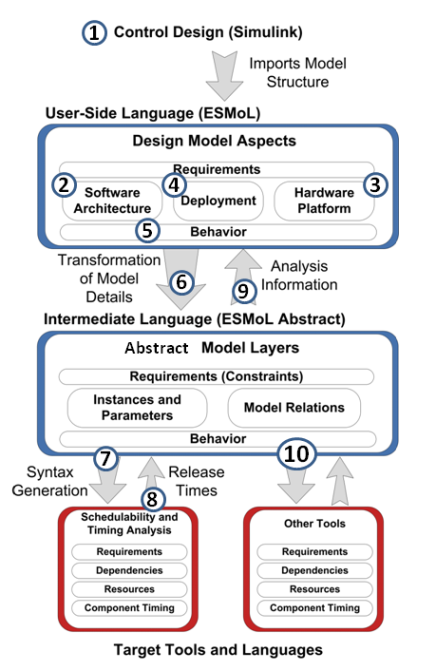
\includegraphics[width=\columnwidth]{figures/designflow.png}
\caption{Design flow supported by the ESMoL language and modeling tools.}
\label{fig:designflow}
\end{figure}

According to \cite{modeling:esmol}, we follow the design flow shown in Fig. \ref{fig:designflow}. Step 1 is to specify the control system's functionality in the Simulink environment. After validation of this control system design, the model can be imported automatically into the ESMoL environment. The Simulink model will become a synchronous dataflow model (SDF), and each subsystem in the Simulink model becomes an actor in the SDF \cite{moc:sdf}. ESMoL model references to imported Simulink blocks become the functional specifications for instances of software components in a logical SDF model. C code fragments may also be used to specify component functionality. Component instance ports (shown in Fig. \ref{fig:QuadrotorLogicalSoftwareArchitecture}) represent instances of data message types. These types are defined as structures with individual data fields to which Simulink data ports can be mapped. These relations describe the marshaling, demarshaling, and transfer of data between software components \cite{modeling:esmol}.

Step 2 is to specify the logical software architecture which captures data dependencies between software component instances independent of their distribution over different processors.

Step 3 is to define hardware platforms hierarchically as hardware units with ports for interconnections. Primitive components include processing nodes and communication buses. Behavioral semantics for these networks models come from the underlying time-triggered architecture. The time-triggered platform provides services such as deterministic execution of replicated components and timed message-passing. Model attributes for hardware also capture timing resolution, overhead parameters for data transfers, and task context switching times \cite{modeling:esmol}. Each element of the platform should have a characterization in terms of performance parameters together with the functionality it can support \cite{modeling:platform}. In ESMoL the performance parameters and the functionality are defined by choosing a hardware unit from \emph{SystemAspect} and setting the \emph{DeviceType} and \emph{Configuration} in \emph{Attribute}.

Step 4 is to set up a deployment model by mapping software components to processing nodes, and data messages to communication ports. The deployment model captures the assignment of component instances as periodic tasks running on a particular processor. In ESMoL a task executes on a processing node at a single periodic rate. All components within the task execute synchronously. Message ports on component instances are assigned to hardware interface ports in the model to define the media through which messages are transferred \cite{modeling:esmol}.

Step 5 is to establish a timing model by attaching timing parameter blocks to components and messages. For the time-triggered case the configuration parameters include execution period and worst-case execution time. The execution model also indicates which components and messages will be scheduled independently, and which will be grouped into a single task or message object \cite{modeling:esmol}.

The TLM scheduling information is added in step 6 through step 9. Step 6 translates an ESMoL model into the simpler ESMoL\_Abstract model using the Stage 1 model transformation described in \cite{modeling:esmol}. Step 7 is to use the equivalent model in ESMoL\_Abstract to generate a scheduling problem specification according to a template. In step 8 a tool called \emph{SchedTool} solves the generated scheduling problem. Step 9 is to import the results back into the ESMoL model and write to the appropriate objects. For more details, please refer to \cite{modeling:esmol}. Step 10 is to generate the corresponding C code, which will be described in next section.


\section{Modeling and Code Generation}

In this case study, we use the above approach to design and implement the embedded software for a quadrotor helicopter. Our example is not distributed, but we are working towards distributed experiments and scenarios involving multiple vehicles. Quadrotor helicopters are agile aircraft which are lifted and propelled by four rotors. Because their attitude dynamics change so quickly, it is difficult if not impossible for a human to successfully fly and maneuver such vehicles \cite{quad:passcontrol}. Thus, these aircraft need an automated control system to help them fly. The controller, software and hardware design domains are highly specialized and conceptually incompatible. For example, control theory deals with a continuous system, software design is for a discrete environment, and computing hardware must deal with both. This makes effectively and efficiently implementing such a high confidence embedded control system significantly difficult. Our embedded software design approach gives a state-of-the-art solution to this.

\subsection{Simulink model of the quadrotor's control system}

The control design for the quadrotor helicopter is introduced in \cite{quad:passcontrol}, which uses passive attitude and altitude control schemes. In the control system of \cite{quad:passcontrol}, two linear proportional derivative (PD) controllers are used, an inner loop and an outer loop. The outer loop controller is a ``fast'' PD inertial controller and the inner loop is a ``fast'' PD attitude controller. \cite{quad:passcontrol} describes the corresponding control approach in detail.

On most quadrotors, the on-board sensors include a GPS and an IMU. In the Simulink model we do not capture the behavior and interfaces of the particular sensor chips, so their receiving message types are modeled not specifically but universally. \cite{quad:passcontrol} takes x, y, and z coordinates instead of longitude, latitude and height as position, so a specific subsystem \emph{Sensor\_Convert} is added to make the conversion. The \emph{Outer\_Loop} subsystem is for inertial position control and \emph{Inner\_Loop} is for attitude control. \emph{Reference\_Handler} is used to receive and handle destinations, and \emph{Plant\_Dynamics} is used to simulate the behavior (not realized as a software component).

\subsection{Logical software architecture of the control system}

\begin{figure}[!t]
\centering
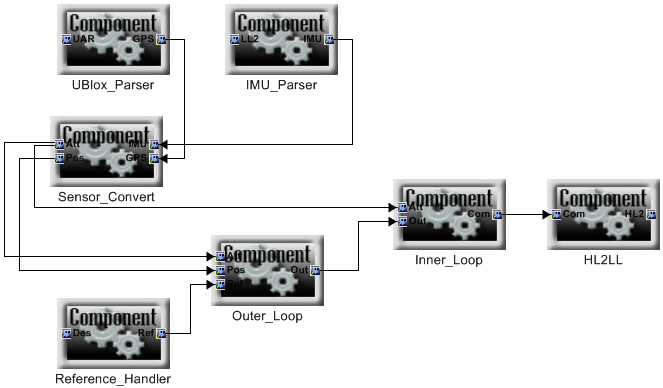
\includegraphics[width=\columnwidth]{figures/QuadrotorLogicalSoftwareArchitecture.png}
\caption{The logical software architecture for quadrotor's control system.}
\label{fig:QuadrotorLogicalSoftwareArchitecture}
\end{figure}

Fig. \ref{fig:QuadrotorLogicalSoftwareArchitecture} shows logical data dependencies between software component instances. There are 7 components needed in this case study. In fact, most of the components' functions are specified by Simulink dataflow diagram. In our case, \emph{Sensor\_Convert}, \emph{Reference\_Handler}, \emph{Inner\_Loop} and \emph{Outer\_Loop} are all specified as Simulink subsystems. SDF is only an abstract MoC to describe data movement semantics for our model, so we must add details regarding specific message structures for the sensors and actuators. We need three components specified by C functions, namely \emph{UBlox\_Parser}, \emph{IMU\_Parser} and \emph{HL2LL}. These three components convert the hardware specific message structures to the message structures required by the Simulink functions.

To determine functional determinism and deadlock freedom, we analyze the imported Simulink blocks in the logical architecture model as a SDF model. SDF guarantees that each actor (corresponding to a subsystem in the Simulink model) can fire at any time only if its input tokens (corresponding to messages) are available on its incoming arcs. In order to extend the execution semantics to include timing determinism while maintaining the benefits of synchronous execution implied by SDF, we employ a time-triggered MoC. On a single processor we use a simple static task schedule without preemption, but we will extend our work to distributed cases.
The time-triggered MoC preserves function determinism and deadlock freedom of the SDF, except that the actors all fire only at the scheduled times.

\subsection{Hardware platform model}

\begin{figure}[!t]
\centering
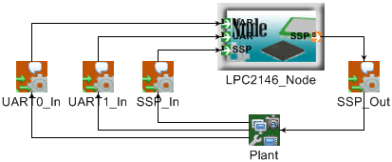
\includegraphics[width=\columnwidth]{figures/QuadrotorHardwarePlatform.png}
\caption{The hardware platform model of AscTec AutoPilot.}
\label{fig:QuadrotorHardwarePlatform}
\end{figure}

The quadrotor helicopter that we use is named AscTec Hummingbird AutoPilot from Ascending Technologies Company \cite{asctech:hummingbird}. The quadrotor's hardware architecture is based on Philips LPC2146. Fig. \ref{fig:QuadrotorHardwarePlatform} illustrates the hardware platform model. The processor LPC2146 is based on an ARM7TDMI-S CPU with two UARTs, SPI, SSP, etc... The peripherals are modeled in the diagram as objects connecting the input and output ports on the processor to the object representing the plant dynamics. A GPS device is connected through UART1, and a Zigbee module used to receive reference is connected via UART0. The IMU and actuators are connected through SSP. Each device can be configured by setting the \emph{Configuration} attribute of the model object representing the device channel. For example, consider the string ''\emph{baudrate = 57600 8n1}`` in the \emph{Configuration} attribute of the channel port connected to device UART0.

\subsection{Deployment model}

\begin{figure}[!t]
\centering
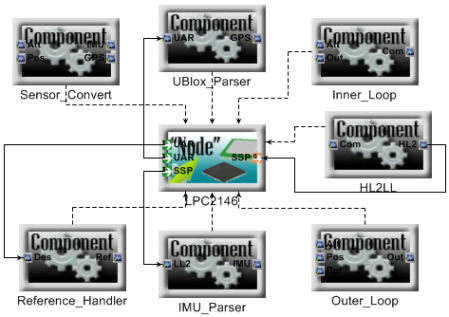
\includegraphics[width=\columnwidth]{figures/QuadrotorDeployment.png}
\caption{The deployment model of control system's software components.}
\label{fig:QuadrotorDeployment}
\end{figure}

In our case study, the model assigns each software component to its own task. In Fig. \ref{fig:QuadrotorDeployment} the dashed connection from a component to a node reference represents an assignment of that component to run as a task on the node. The port connections represent the hardware channel through which that particular message will travel. Local data dependencies are not specified here, as they are represented in the logical software architecture. IChan and OChan objects on the node can also be connected to message objects on a component. These connections represent the flow of data from the physical environment through sensors (IChan objects) or the flow of data back to the environment through actuators (OChan objects).

\subsection{Timing model}

\begin{figure}[!t]
\centering
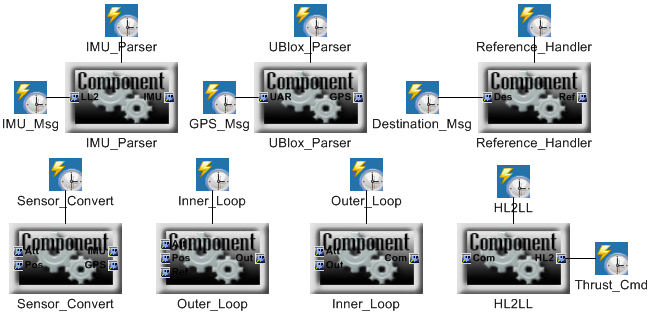
\includegraphics[width=\columnwidth]{figures/QuadrotorTimingModel.png}
\caption{The timing model of each software component and communication channel.}
\label{fig:QuadrotorTimingModel}
\end{figure}

The global period (and deadline) is 1 ms, as that is the fundamental sampling rate of the hardware. The worst case latency from sensors to actuators must be smaller than the given timing requirement. In Fig. \ref{fig:QuadrotorTimingModel}, each component is assigned a \emph{TTExecInfo} (Time-Triggered Execution Information) object, so is each external data transfer. The processor-local data transfers transfer time is neglected, as reads and writes occur in locally shared memory. The quadrotor is controlled at 1kHz, so the \emph{ExecPeriod} attribute for all components except for \emph{Blox\_Parser} is 1 millisecond. Because the time between two valid data of GPS is longer than 1 millisecond, the \emph{ExecPeriod} for \emph{Blox\_Parser} is 100 milliseconds. Local message transfers may be specified as time-triggered, but in practice they taking place in shared memory are not scheduled. In ESMoL only distributed messages may be scheduled.

\subsection{Code generation}

In order to generate the C code based on the TLM in ESMoL, two interpreters are used, which are in Stage 1 and Stage 2 respectively. The Stage 1 interpreter transforms the TLM to an equivalent model in an intermediate language called ESMoL\_Abstract. The model in this intermediate language is flattened and the relationships implied by structures in ESMoL are represented by explicit relation objects in ESMoL\_Abstract \cite{modeling:esmol}.

Stage 2 provides several interpreters, each of which uses the UDM model navigation API to translate the ESMoL\_Abstract model into either code or an analysis model. The deployment model objects are used to generate platform-specific task wrapping and communication code. Shared memory is used to implement the message passing through the ports.

The code generator uses the Google CTemplate engine called from C++ code to perform the generation tasks. We establish a template library containing the initialization codes of different devices. This makes the control system code able to be used on different platforms with a variety of different sensors and actuators. Using the idea of separately generating functional and platform specific code is to realize the platform-based design concept. The functional code implements the individual component behaviors, and the wrappers implement the component interactions.

Real-Time Workshop (RTW) generates functional ANSI C code for the subsystems specified as Simulink blocks.

Due to the lack of an operating system, we use interrupt-based multi-tasking. The timer interrupt service routine invokes the tasks according to the specified schedule.


\section{Evaluation}

We emperically evaluate the execution time for each component using an external indicator, and timing requirements of these components are met. Each of them takes less than 10 us during normal operation.

The memory system consists of 256KB on-chip flash memory (ROM) and 32KB SRAM (RAM). The corresponding binary code is about 130KB, so it fits in the system's ROM space. We also emperically evaluate that the RAM space is enough for data during normal operation. Since all the data variables for the communication are preallocated, this memory evaluation will not change in any cases.

\section{Future work}

Our future work includes: 1) multiple quadrotor helicopters control approach design and corresponding embedded software design 2) distributed experiments 3) fixed-point function generation 4) time-triggered wireless network.



% use section* for acknowledgement
\section*{Acknowledgment}

National Science Foundation (grant/contract number NSF-CCF-0820088), Air Force Office of Scientific Research, USAF (grant/contract number FA9550-06-0312).  

% trigger a \newpage just before the given reference
% number - used to balance the columns on the last page
% adjust value as needed - may need to be readjusted if
% the document is modified later
%\IEEEtriggeratref{8}
% The "triggered" command can be changed if desired:
%\IEEEtriggercmd{\enlargethispage{-5in}}

% references section

% can use a bibliography generated by BibTeX as a .bbl file
% BibTeX documentation can be easily obtained at:
% http://www.ctan.org/tex-archive/biblio/bibtex/contrib/doc/
% The IEEEtran BibTeX style support page is at:
% http://www.michaelshell.org/tex/ieeetran/bibtex/
%\bibliographystyle{IEEEtran}
% argument is your BibTeX string definitions and bibliography database(s)
%\bibliography{IEEEabrv,../bib/paper}
%
% <OR> manually copy in the resultant .bbl file
% set second argument of \begin to the number of references
% (used to reserve space for the reference number labels box)
%\begin{thebibliography}{1}

%\bibitem{IEEEhowto:kopka}
%H.~Kopka and P.~W. Daly, \emph{A Guide to \LaTeX}, 3rd~ed.\hskip 1em plus
%  0.5em minus 0.4em\relax Harlow, England: Addison-Wesley, 1999.

%\end{thebibliography}

\bibliographystyle{IEEEtran}
\bibliography{iccps11}


% that's all folks
\end{document}


